\documentclass[t, screen, aspectratio=43]{beamer}
\usepackage[T1]{fontenc}
\usepackage[utf8]{inputenc}
\usepackage{epsf}
\usepackage{graphicx}
\usepackage{geometry}
\usepackage{tabularx}
\usepackage[table]{colortbl}
\usepackage{xcolor}
\usepackage{soul}
\usepackage[normalem]{ulem}
\usepackage{tikz}
\usepackage{subcaption}
% Use the NTNU-temaet for beamer 
% \usetheme[style=ntnu|simple|vertical|horizontal, 
%     language=bm|nn|en, 
%     smalltitle, 
%     city=all|trondheim|alesund|gjovik]{ntnu2017}
\usetheme[style=helvet,language=en]{ntnu2017}

\usepackage[english]{babel}
\usepackage[style=numeric,backend=biber,natbib=false,sorting=none]{biblatex}

\title[Short title]{Python Framework for Design and Analysis of Integer-N ADPLLs}
\subtitle{Specialization Project Progress - 11th Week}
\author[C Nielsen]{Cole Nielsen}
\institute[NTNU]{Department of Electronic Systems, NTNU}
\date{8 November 2019 (Calendar week 45)}
%\date{} % To have an empty date

\addbibresource{example.bib} % Add bibliography database

% Set the reference style to numeric.
% See here: http://tex.stackexchange.com/questions/68080/beamer-bibliography-icon
\setbeamertemplate{bibliography item}[text] 

% Set bibliography fonts to a small size.
\renewcommand*{\bibfont}{\footnotesize}




\begin{document}

\begin{frame}
	\titlepage%
\end{frame}

% Alternatively, special title page command to get a different background
% \ntnutitlepage

% #############################################################################
% Timeline
% #############################################################################

\begin{frame}
	\frametitle{Timeline}
	\begin{table}[htb!]
		\tiny
		\centering
		\vspace{-1em}
		\def\arraystretch{1.5}		
		\setlength\arrayrulewidth{0.75pt}
		\setlength{\tabcolsep}{1em} % for the horizontal padding
		\begin{tabular}{|l|l|l|l|}
			\hline 
			\rule[-1ex]{0pt}{2.5ex} \cellcolor{gray!40}\textbf{Week} & \cellcolor{gray!40}\textbf{Dates} &\cellcolor{gray!40}\textbf{Tasks} & \cellcolor{gray!40}\textbf{Outcomes}\\ 
			\hline 
			\rule[-1ex]{0pt}{2.5ex} \cellcolor{red!20}\textbf{36}& \cellcolor{red!20}2.9 - 8.9 & \cellcolor{red!20}Review PLL Design & \cellcolor{red!20}Refreshed Knowledge\\ 
			\hline 
			\rule[-1ex]{0pt}{2.5ex} \cellcolor{red!20}\textbf{37}& \cellcolor{red!20}9.9 - 15.9 & \cellcolor{red!20}Modeling/simulation (set up) & \cellcolor{red!20}--\\ 
			\hline 
			\rule[-1ex]{0pt}{2.5ex} \cellcolor{red!20}\textbf{38}& \cellcolor{red!20}16.9 - 22.9 & \cellcolor{red!20}Modeling/simulation &\cellcolor{red!20}TDC/DCO Requirements\\ 
			\hline 
			\rule[-1ex]{0pt}{2.5ex} \cellcolor{red!20}\textbf{39}& \cellcolor{red!20}23.9 - 29.9& \cellcolor{red!20}Modeling/simulation& \cellcolor{red!20}Loop Filter/Digital Algorithms\\ 
			\hline 
			\rule[-1ex]{0pt}{2.5ex} \cellcolor{red!20}\textbf{40}& \cellcolor{red!20}30.9 - 6.10& \cellcolor{red!20}Modeling/simulation& \cellcolor{red!20}{Loop filter, DCO, TDC, calibration}\color{black}\\ 
			\hline 
			\rule[-1ex]{0pt}{2.5ex} \cellcolor{red!20}\textbf{41}&\cellcolor{red!20}7.10 - 13.10&\cellcolor{red!20}Circuit Research &\cellcolor{red!20}DCO/Divider topologies\\ 
			\hline 
			\rule[-1ex]{0pt}{2.5ex} \cellcolor{red!20}\textbf{42}&\cellcolor{red!20}14.10 - 20.10&\cellcolor{red!20}Circuit Research &\cellcolor{red!20}TDC/other topologies\\ 
			\hline 
			\rule[-1ex]{0pt}{2.5ex} \cellcolor{red!20}\textbf{43}&\cellcolor{red!20}21.10 - 27.10&\cellcolor{red!20}Spur analysis, filter automation &\cellcolor{red!20} \\ 
			\hline 
			\rule[-1ex]{0pt}{2.5ex} \cellcolor{red!20}\textbf{44}&\cellcolor{red!20}28.10 - 3.11&\cellcolor{red!20}Filter automation, SNR estimation&\cellcolor{red!20}\\ 
			\hline 
			\rule[-1ex]{0pt}{2.5ex} \cellcolor{green!20}\textbf{45}&\cellcolor{green!20}4.11 - 10.11&\cellcolor{green!20}Variation analysis, flicker noise &\cellcolor{green!20}Histograms/yield estimates\\ 
			\hline 
			\rule[-1ex]{0pt}{2.5ex} \textbf{46}& 11.11 - 17.11& Real DCO sensitivity, TDC/divider jitter& Simlate ring-DCO in Virtuoso\\ 
			\hline 
			\rule[-1ex]{0pt}{2.5ex} \textbf{47}& 18.11 - 24.11& PLL + Radio simulation& BER estimate\\ 
			\hline 
			\rule[-1ex]{0pt}{2.5ex} \textbf{48}& 25.11 - 1.12& Agglomerate into cohesive framework & (I have an Exam on 30.11)\\ 
			\hline 
			\rule[-1ex]{0pt}{2.5ex} \textbf{49}& 2.12 - 8.12& Finish framework, report writing& \\ 
			\hline 
			\rule[-1ex]{0pt}{2.5ex} \textbf{50}& 9.12 - 15.12& Report writing& Complete before 15.12\\ 
			\hline 
		\end{tabular}
		\begin{flushleft}\textbf{Legend:} \colorbox{red!20}{\textbf{Done}} \colorbox{green!20}{\textbf{Current}}  \colorbox{blue!20}{\textbf{Revised}}
		% *I will write the report simultaneously with the work.
		\end{flushleft}
		% \caption{Assigned specifications for branch line hybrid design.}
		% \label{asgn_specs}
	\end{table}   
\end{frame}


% #############################################################################
% This week
% #############################################################################

\begin{frame}
	\frametitle{Timeline Tasks}
	\begin{block}{This week}
		\begin{itemize}
			\footnotesize
			\item \textbf{Loop filter optimization:}
			\begin{itemize}
				\footnotesize
				\item Devised new method to optimize loop filter based on lock-time and total phase noise power estimates of loop filter.
			\end{itemize} 
			\item \textbf{Variation/sweep analysis}:
			\begin{itemize}
				\footnotesize
				\item Implemented engine for parametric sweep and variation analysis through Monte-Carlo sampling.
				\begin{itemize}
					\scriptsize
					\item Can easily vary an arbitrary number of parameters.
					\item Utilize parallelization across CPU cores for speed.
				\end{itemize}			
				\item Yield estimate based on statistical fits of data, can also emulate corner cases. 
			\end{itemize} 
		\end{itemize}    
	\end{block}
\end{frame}

% #############################################################################
% sim/modeling approach
% #############################################################################

\begin{frame}
	\frametitle{Filter automation}
	\begin{block}{So, what is truly optimal???}
			\center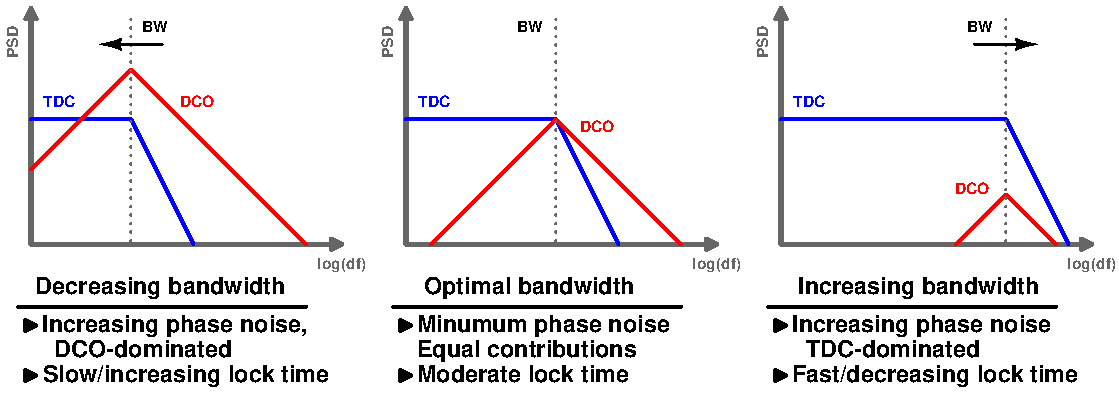
\includegraphics[width=0.8\textwidth, angle=0]{loop_bandwidth.pdf}
		\begin{itemize}
			\scriptsize
			\item Optimal phase noise occurs when TDC/DCO contributions are approximately equal. 
			\begin{itemize}
				\scriptsize
				\item However this may not occur at a wide enough bandwidth for desired lock time.
			\end{itemize}
			\item Therefore optimum is when:
			\begin{itemize}
				\scriptsize
				\item Total phase noise is minimized \textit{while} meeting constraint for maximum lock time.
				\item May have to accept worse phase noise to achieve lock time.
			\end{itemize}

		\end{itemize}    
	\end{block}
\end{frame}


\begin{frame}
	\frametitle{Filter automation}
	\begin{block}{New optimization approach}
		\begin{itemize}
			\scriptsize
			\item Constrained by a maximum settling time $t_{s,max}$, try to minimize phase noise.
			\begin{itemize}
				\scriptsize
				\item Utilize quick estimates in optimizer of \textbf{(a)} integrated phase noise power and \textbf{(b)} settling time of PLL for an arbitrary closed loop response G(f).
			\end{itemize}
			\item \textbf{Phase noise estimate}
			\begin{itemize}
				\scriptsize
				\item Use same models as before for phase noise of PLL, where $S_{TDC}$ and $S_{DCO}$ are the intrinsic phase noise PSD respectively for the TDC and DCO. N is the PLL divider modulus. The total PLL phase noise $S_{\Sigma}(f)$ is:
				\begin{equation}
				S_{\Sigma}(f) = f_{clk}\cdot|2\pi N\cdot G(f)|^2S_{TDC} + |1-G(f)|^2S_{DCO}
				\end{equation}
				\item Given a bandwidth of interest $\Delta f$ (i.e. baseband bandwidth), the total integrated phase noise power is:
				\begin{equation}
				P_{\phi noise} = 2\int_0^{\Delta f} S_{\Sigma}(f)df
				\end{equation}

			\end{itemize}
		\end{itemize}    
	\end{block}
\end{frame}

\begin{frame}
	\frametitle{Filter automation}
	\begin{block}{New optimization approach}
		\begin{itemize}
			\scriptsize
			\item \textbf{Settling time (PLL lock time) estimate}
			\begin{itemize}
				\tiny
				\item Easy to translate G(f) to state space representation with Python (\texttt{scipy.special)}:
				\tiny
				\begin{equation}
				G(f) = \frac{\Sigma_0^M b_ms^m}{\Sigma_0^N a_ns^n} \hspace{1em} \rightarrow \hspace{1em} s\mathbf{Y}(s) = \mathbf{AY}(s) +\mathbf{B}X(s)
				\end{equation}
				\item The state transition matrix is then $\boldsymbol{\Phi} = (s\mathbf{I}-A)^{-1}$. The eigenvalues and eignvectors of $\boldsymbol{\Phi}$ are then $\{\lambda_1, ... , \lambda_{N}\}$ and $\{\mathbf{v}_1, ... , \mathbf{v}_N\}$ respectively. The step response of G(f) takes the form:
				\begin{equation}
				\mathbf{y}(t) = \mathbf{v_1}e^{\lambda_1t} + ... + \mathbf{v_k}e^{\lambda_kt}, \hspace{1em} \mathbf{y}(t) = [ y(t) \hspace{0.5em}y^{'}(t)\hspace{0.5em} ...\hspace{0.5em} y^{(k)}(t)]^T
				\end{equation}
				\item The $\lambda_k$ with the smallest real component then governs the long term settling of y(t). Assuming one dominant pole, the time constant of G(f) can be estimated as $\Re(\lambda_k)^{-1}$. Settling time $t_s$ can be considered as the interval required for the signal to drop within a tolerance band $\pm \delta_{tol} \textnormal{y}(\infty)$ about the final value y$(\infty)$. Thus:
				\begin{equation}
				t_s = \tau\ln(\delta_{tol}) = \frac{\ln(\delta_{tol})}{\min(|\Re(\{\lambda_1, ... , \lambda_k\})|)}
				\end{equation}
				\item This turns out to be fairly accurate versus simulation.
			\end{itemize}
		\end{itemize}    
	\end{block}
\end{frame}

\begin{frame}
	\frametitle{Filter automation}
	\begin{block}{New optimization approach}
		\begin{itemize}
			\scriptsize
			\item Based on the open loop PLL transfer function A(f), optimization for the closed loop G(f) is done using two levels of optimization.
			\begin{equation}
				A(f) = \frac{K}{s^2}\frac{(s/\omega_z +1)}{(s/\omega_p +1)}
			\end{equation}
			\item \textbf{Level A - Minimize phase noise for fixed settling time.}
			\begin{itemize}
				\scriptsize
				\item Minimize phase noise while maintaining fixed settling time = $t_s$.
				\item \textbf{Solution:} use two steps per interation until satisfactorily converged:
				\begin{enumerate}
					\scriptsize
					\item Minimize phase noise using pole/zeros locations (gradient descent).
					\item Tune K such that settling time = $t_s$ (golden section search).
				\end{enumerate}

			\end{itemize}
		\item \textbf{Level B - Optimize settling time given constraints.}
		\begin{itemize}
			\scriptsize
			\item Use golden section search to find optimal constrained settling time that has minimal phase noise using method from level A as cost function.
		\end{itemize} 
		\end{itemize}    
	\end{block}
\end{frame}



\begin{frame}
	\frametitle{Variation analysis}
	\begin{block}{Monte-Carlo sampling }
		\begin{itemize}
		\scriptsize
		\item Implemented analysis of variaton using Monte-Carlo (MC) sampling.
		\item Simulation configured by dictionary with PLL/simulation parameters. 
		\begin{itemize}
			\scriptsize
			\item Implemented MC engine allows for variation any of these parameters, or any combination of the parameters.
		\end{itemize}
		\item Implemented concurent execution of simulations with \texttt{multiprocessing} package.
		\begin{itemize}
			\scriptsize
			\item Can run 8 simulations simultaneously on my machine
			\item Run of 1000 simulations for Monte-Carlo analysis of settling time takes ca. 20s.
		\end{itemize}
		\end{itemize}    
	\end{block}
\end{frame}

\begin{frame}
	\frametitle{Variation analysis}
	\begin{block}{Monte-Carlo sampling }
		\begin{itemize}
		\scriptsize
		\item \textbf{Example 1 - KDCO variation}
		\begin{itemize}
			\scriptsize
			\item $f$=2.4 GHz, $f_{ref}$=16 MHz, 150 TDC steps, 20ps BBPD resolution, KDCO = 10 kHz/LSB, $\sigma_{KDCO}$ = 2 kHz, initial $f_{error}$ = 12 MHz.
			\item Settling/lock tolerance = $\pm 100 kHz$, samples = 1000
		\end{itemize}
		\center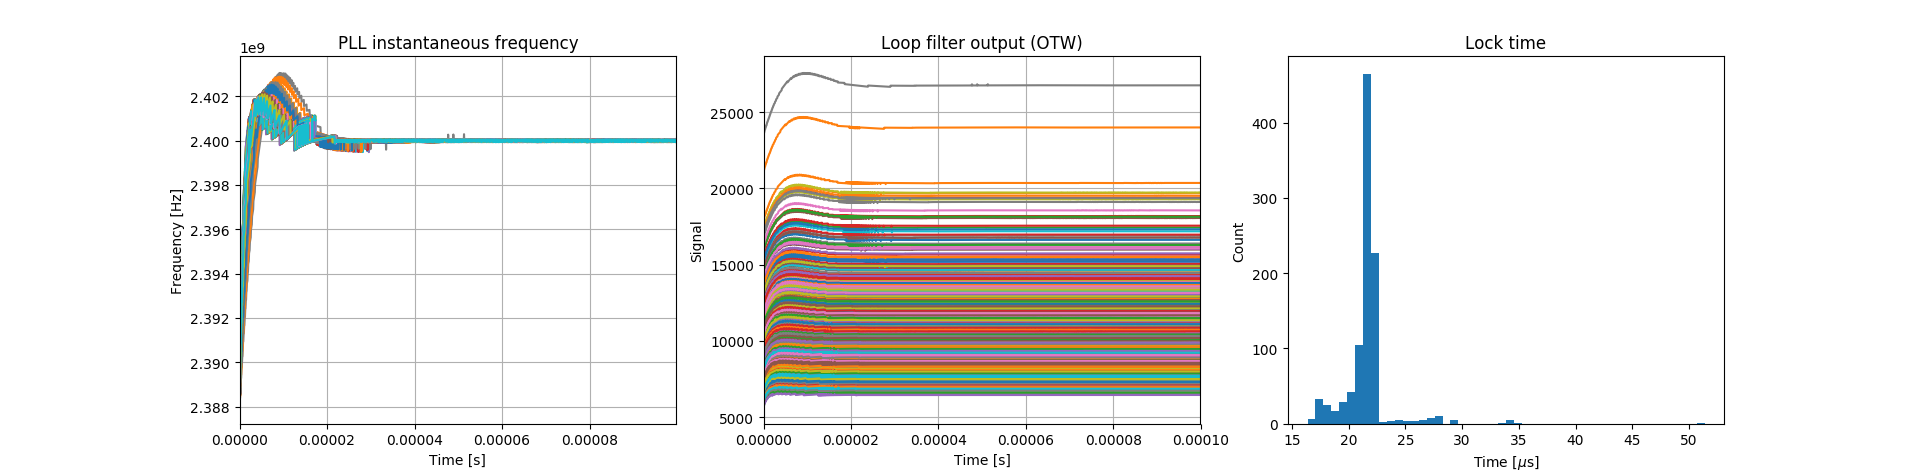
\includegraphics[width=1.0\linewidth]{kdco_mc_hist.png}
		\begin{itemize}
			\scriptsize
			\item Mean = 34.2 $\mu$s
			\item Non-gaussian distribution
		\end{itemize}

		\end{itemize}    
	\end{block}
\end{frame}

\begin{frame}
	\frametitle{Variation analysis}
	\begin{block}{Monte-Carlo sampling }
		\begin{itemize}
		\scriptsize
		\item \textbf{Example 1 - KDCO variation + large initial frequency variation }
		\begin{itemize}
			\scriptsize
			\item $f$=2.4 GHz, $f_{ref}$=16 MHz, 150 TDC steps, 20ps BBPD resolution, KDCO = 10 kHz/LSB, $\sigma_{KDCO}$ = 2 kHz, initial frequency error $\sigma_{f-error}$ = 5 MHz.
			\item Settling/lock tolerance = $\pm 100 kHz$, samples = 1000
		\end{itemize}
		\center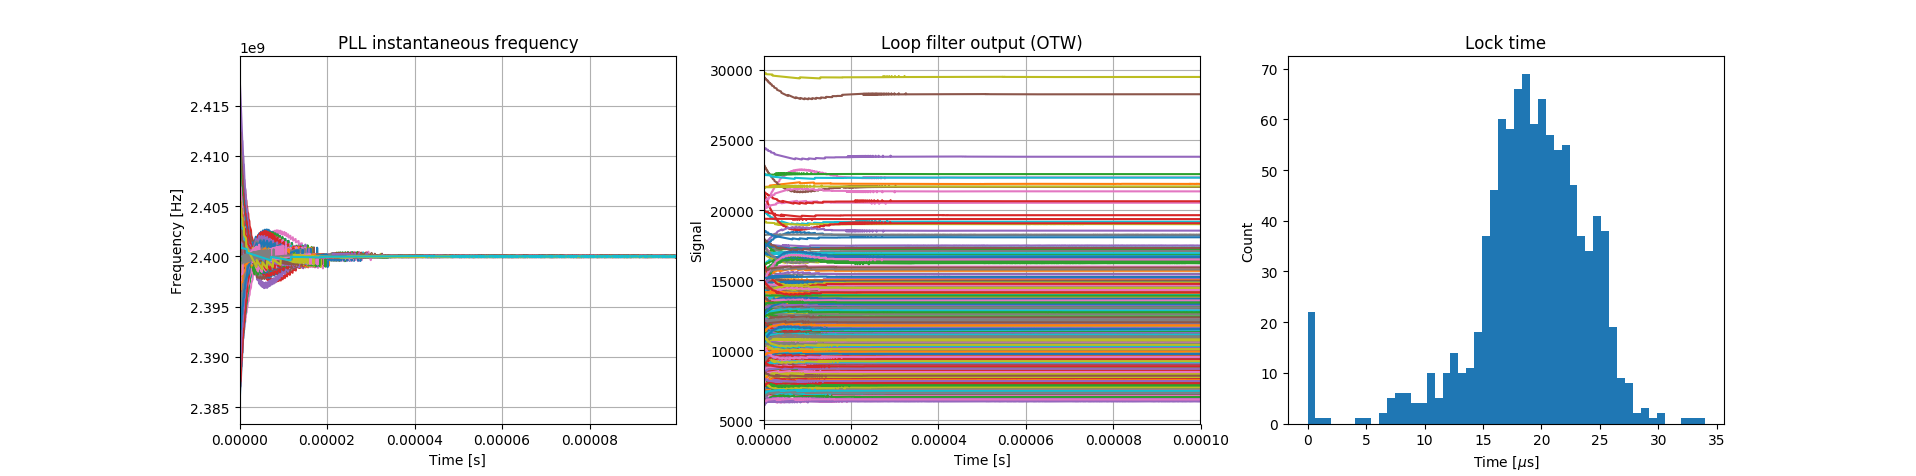
\includegraphics[width=1.0\linewidth]{kdco_f_init_mc_hist.png}
		\center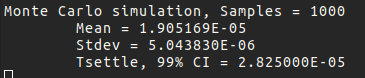
\includegraphics[width=0.4\linewidth]{mc_large_df.png}

		\end{itemize}    
	\end{block}
\end{frame}

\begin{frame}
	\frametitle{Variation analysis}
	\begin{block}{Monte-Carlo sampling }
		\begin{itemize}
		\scriptsize
		\item \textbf{Example 1 - KDCO variation + small initial frequency variation }
		\begin{itemize}
			\scriptsize
			\item $f$=2.4 GHz, $f_{ref}$=16 MHz, 150 TDC steps, 20ps BBPD resolution, KDCO = 10 kHz/LSB, $\sigma_{KDCO}$ = 2 kHz, initial frequency error  $\sigma_{f-error}$ = 0.25 MHz.
			\item Settling/lock tolerance = $\pm 100 kHz$, samples = 1000
		\end{itemize}
		\center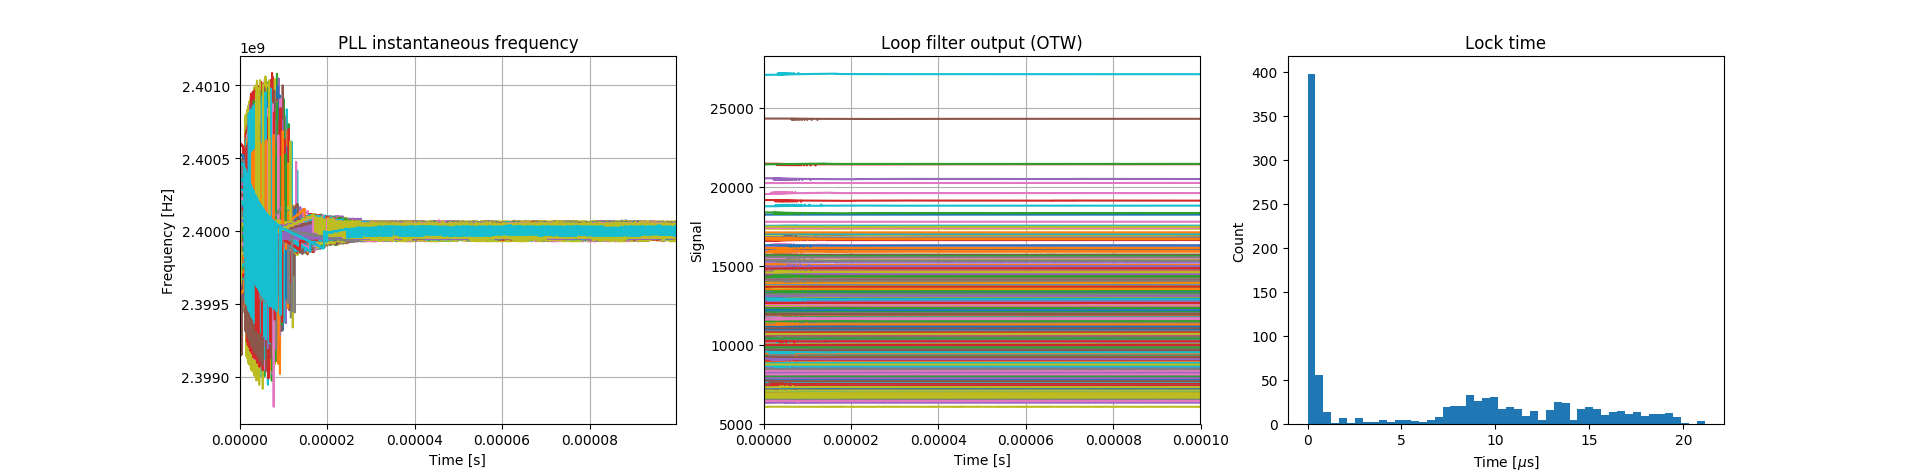
\includegraphics[width=1.0\linewidth]{kdco_small_df_f_init_mc_hist.png}
		\center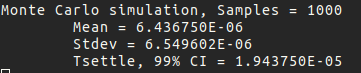
\includegraphics[width=0.4\linewidth]{mc_small_df.png}

		\end{itemize}    
	\end{block}
\end{frame}

\begin{frame}
	\frametitle{Variation analysis}
	\begin{block}{Monte-Carlo sampling }
		\begin{itemize}
		\scriptsize
		\item It should be noted that the mean lock time from the large initial frequency deviation simulation (19.1 $\mu$s) to the small frequency deviation simulation (6.4 $\mu$s) decreased.
		\item This implies the lock-time (i.e. re-lock time) improvement with the ADPLL for starting with a small frequency error desired for use with a WuRx is realized.
		\begin{itemize}
			\scriptsize
			\item Further improvements in re-lock time should be realizable through optimization.
			\item Should enable power reduction in WuRx versus analog PLL due to this lock time improvement.
		\end{itemize}
		\end{itemize}    
	\end{block}
\end{frame}

\begin{frame}
	\frametitle{Variation analysis}
	\begin{block}{Parameter sweeps}
		\begin{itemize}
		\scriptsize
			\scriptsize
			\item Can sweep arbitiary PLL/simulation parameters in similar fashion to MC simulation.
			\item $f$=2.4 GHz, $f_{ref}$=16 MHz, 150 TDC steps, 20ps BBPD resolution, KDCO = [2,18] kHz/LSB, initial frequency error = 12 MHz.
			\item Settling/lock tolerance = $\pm 100 kHz$, samples = 11
		\end{itemize}    
		\center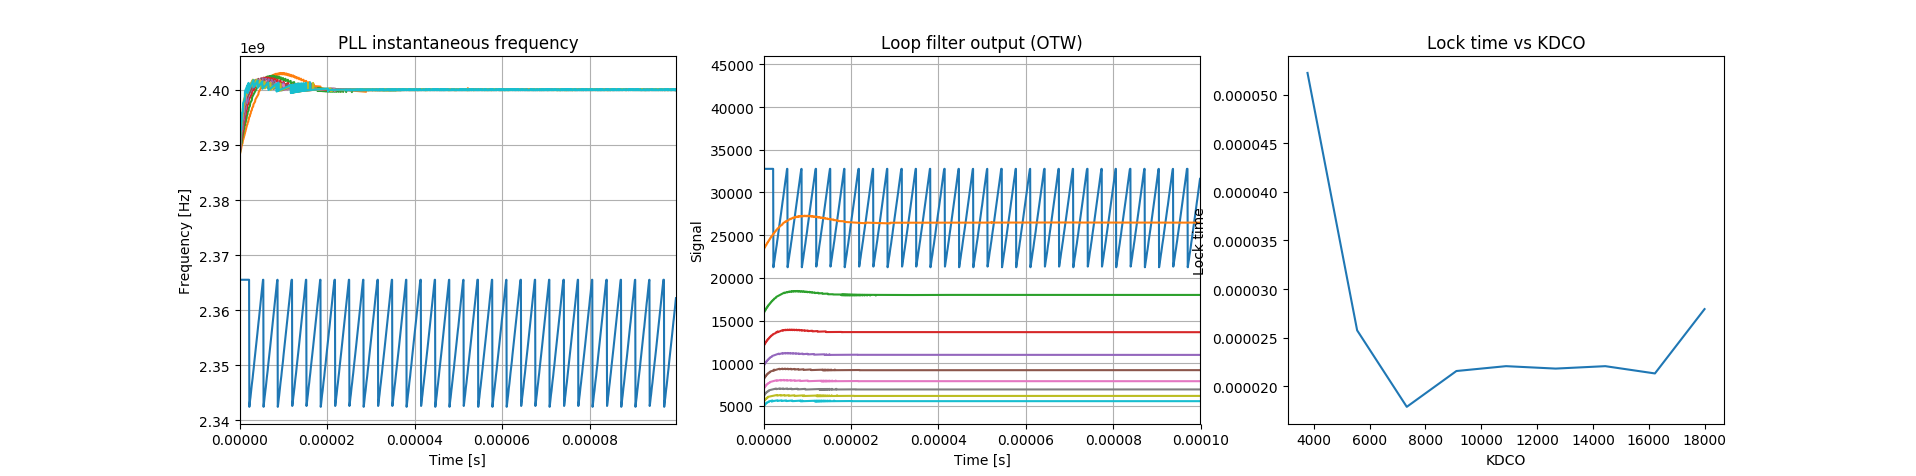
\includegraphics[width=1.0\linewidth]{sweep.png}
	\end{block}
\end{frame}



% #############################################################################
% Loop Dynamics (continuous)
% #############################################################################

% \begin{frame}
% 	\frametitle{Loop Dynamics}
% 	\begin{block}{Still To Do}
% 		\vspace{-.2em}
% 		\begin{itemize}
% 			\footnotesize
% 			\item Standard approach to used mixed continuous/discrete time mathematical model for DPLL. 
% 			\item Plot of RO phase noise (typical)
% 			\item Automatic analysis of performance (lock detection, residual phase modulation, lock-in/pull-in range).
% 			\item Automatic optimization (using gradient descent) of PLL parameters?
% 			\item Z-domain modeling of loop? Develop (by hand) some ideal transfer funtions for loop.

% 		\end{itemize}    
% 	\end{block}
% \end{frame}

% #############################################################################
% Specification
% #############################################################################

\begin{frame}
	\frametitle{Specification (unchanged)\color{black}}
	\begin{block}{System Performance Targets}
		\scriptsize
		\begin{table}[h!]
			\centering
			\def\arraystretch{1.5}		
			\setlength\arrayrulewidth{0.75pt}
			\setlength{\tabcolsep}{1em} % for the horizontal padding
			\begin{tabular}{|l|r|l|l|}
				\hline 
				\rule[-1ex]{0pt}{2.5ex} \cellcolor{gray!40}\textbf{Parameter} & \cellcolor{gray!40}\textbf{Value} & \cellcolor{gray!40}\textbf{Unit }& \cellcolor{gray!40}\textbf{Notes}\\ 
				\hline 
				\rule[-1ex]{0pt}{2.5ex} \textbf{Frequency}  & 2.4-2.4835 & GHz & 2.4G ISM Band\\ 
				\hline 
				\rule[-1ex]{0pt}{2.5ex} \textbf{Ref. frequency} & 16 & MHz & Yields 6 channels \\ 
				\hline 
				\rule[-1ex]{0pt}{2.5ex} \textbf{Power} & $\leq$ 100  &$\mu$W & \\ 
				\hline 
				\rule[-1ex]{0pt}{2.5ex} \textbf{FSK BER} & $\leq$ 1e-2  & & 2FSK with $f_{dev}$=$\pm$250 KHz\\ 
				\hline 
				\rule[-1ex]{0pt}{2.5ex} \textbf{Initial Lock Time} & $\leq$ 50 & $\mu$s & Upon cold start \\ 
				\hline 
				\rule[-1ex]{0pt}{2.5ex} \textbf{Re-lock Time} & $\leq$ 5 & $\mu$s & Coming out of standby \\ 
				\hline 
				\rule[-1ex]{0pt}{2.5ex} \textbf{Bandwidth} & 50 & kHz & (nominally), tunable \\ 
				\hline 
			\end{tabular} 
			% \caption{Assigned specifications for branch line hybrid design.}
			% \label{asgn_specs}
		\end{table}   
		Additionally: PLL output should support IQ sampling at LO frequency.
	\end{block}    
\end{frame}

\begin{frame}
	\frametitle{Specification (unchanged)}
	\begin{block}{PLL Component Performance Targets}
		\scriptsize
		\begin{table}[h!]
			\centering
			\def\arraystretch{1.5}		
			\setlength\arrayrulewidth{0.75pt}
			\setlength{\tabcolsep}{1em} % for the horizontal padding
			\begin{tabular}{|l|r|l|l|}
				\hline 
				\rule[-1ex]{0pt}{2.5ex} \cellcolor{gray!40}\textbf{Parameter} & \cellcolor{gray!40}\textbf{Value} & \cellcolor{gray!40}\textbf{Unit }& \cellcolor{gray!40}\textbf{Notes}\\ 
				\hline 
				\rule[-1ex]{0pt}{2.5ex} \textbf{DCO LSB Resolution}  & $\leq$ 50  & kHz & Determined from quantization noise.\\ 
				\hline 
				\rule[-1ex]{0pt}{2.5ex} \textbf{DCO DNL} & < 1 & LSB & Ensures monotonicity \\ 
				\hline 
				\rule[-1ex]{0pt}{2.5ex} \textbf{TDC Resolution} & 0.95  & ns & \\ 
				\hline 
				\rule[-1ex]{0pt}{2.5ex} \textbf{TDC Resolution (bits)} &  6 &bits & \\ 
				\hline 
			\end{tabular} 
			% \caption{Assigned specifications for branch line hybrid design.}
			% \label{asgn_specs}
		\end{table}   
	\end{block}    
\end{frame}

% #############################################################################
% Architecture - block diagram
% #############################################################################

\begin{frame}
	\frametitle{Architecture (updated)}
	\begin{block}{Block Diagram}
	\center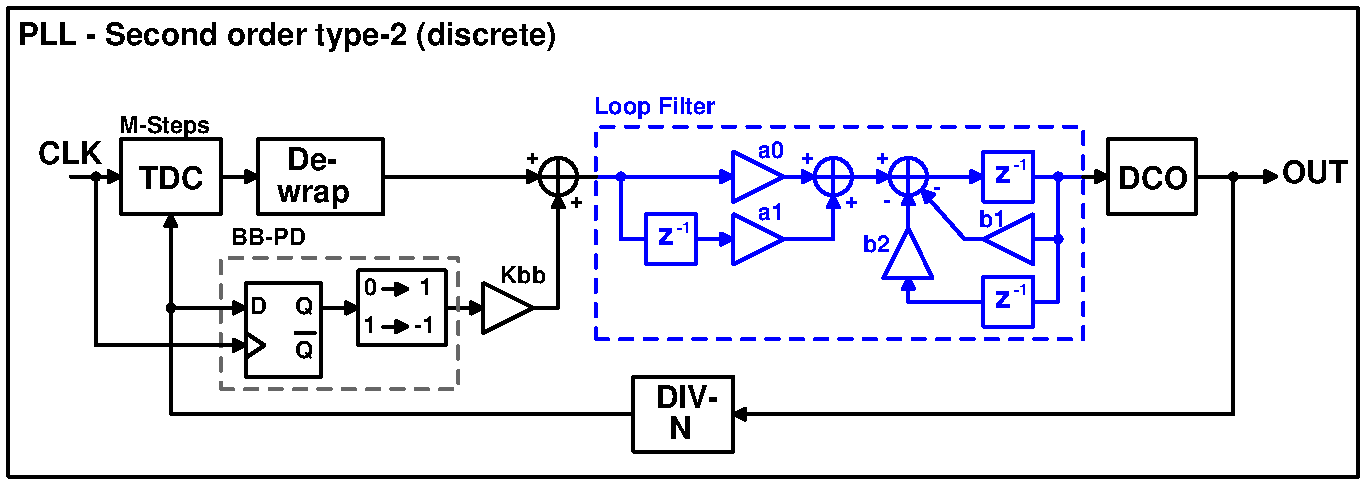
\includegraphics[width=0.8\textwidth, angle=0]{pll_sec_order_bb.pdf}

	\end{block}
		\begin{block}{Power Targets}
		\vspace{-.1em}
		\begin{table}[htb!]
			\tiny
			\centering
			\def\arraystretch{1.5}		
			\setlength\arrayrulewidth{0.75pt}
			\setlength{\tabcolsep}{1em} % for the horizontal padding
			\begin{tabular}{|l|l|l|l|l|}
				\hline 
				\rule[-1ex]{0pt}{2.5ex} \cellcolor{gray!40}\textbf{DCO} & \cellcolor{gray!40}\textbf{TDC} & \cellcolor{gray!40}\textbf{Divider }& \cellcolor{gray!40}\textbf{Other} & \cellcolor{gray!40}\textbf{SUM} \\ 
				\hline 
				\rule[-1ex]{0pt}{2.5ex} 70 $\mu$W& 20 $\mu$W & 10 $\mu$W & $<<$ 1 $\mu$W & 100 $\mu$W\\ 
				\hline 
			\end{tabular} 
			% \caption{Assigned specifications for branch line hybrid design.}
			% \label{asgn_specs}
		\end{table}   
	\end{block}

\end{frame}


% #############################################################################
% project phases
% #############################################################################


\begin{frame}
	\frametitle{Project Phases}
	\begin{block}{Autumn 2019}
		\footnotesize
		\begin{itemize}
			\item System modeling and simulation.
			\begin{itemize}
				\footnotesize
				\item Learn PLL theory in detail
				\item Evaluate feasability of PLL architectures (counter, TDC-based)
				\item Determine requirements for TDC/DCO/Divider/logic (bits of resolution, accuracy etc) to meet PLL performance specifications.
				\item Determine digital logic for loop filter, validate stability and lock time performance.
			\end{itemize}
			\item Research ultra-low power circuit topologies to implement system components that will meet determined requirements.
			\item Translate component-level specifications into schematic-level circuit designs.
			\begin{itemize}
				\footnotesize
				\item Try, fail, try again until functional at schematic level.
				\begin{itemize}
					\footnotesize
					\item I expect the TDC to be difficult.
				\end{itemize}
			\end{itemize}      
		\end{itemize}
	\end{block}
\end{frame}

% #############################################################################
% Project phases slide 2
% #############################################################################


\begin{frame}
	\frametitle{Project Phases (continued)}
	\begin{block}{Spring 2020}
		\begin{itemize}
			\footnotesize
			\item Finalize schematic-level design.
			\item Estabilish thorough tests for PLL performance (automated?) to help in layout.
			\item Layout of PLL.
			\begin{itemize}
				\footnotesize
				\item Design iteration until design specs met.
				\item Probably very time consuming.
			\end{itemize}
			\item Full characterization/validation of design performance. 
			\begin{itemize}
				\footnotesize
				\item Comprehensive Corners/Monte-Carlo testing (time consuming??)
				\item More design iteration if new issues crop up...
			\end{itemize}
			\item Thesis paper writing.
		\end{itemize}
	\end{block}
\end{frame}

% #############################################################################
% References
% #############################################################################


\begin{frame}
	\frametitle{References}
		\scriptsize
		[1] "Ultra-Low Power Wake-Up Receivers for Wireless Sensor Networks", N. Pletcher, J.M Rabaey, 2008.\\
		\hspace{16pt}\url{http://www.eecs.berkeley.edu/Pubs/TechRpts/2008/EECS-2008-59.html}\\
		\vspace{1em}
		% [2] "Minimum Achievable Phase Noise of RC Oscillators",
	% Navid et al. 2005
\end{frame}


\end{document}
